%   % !TEX root = ../../VIII,3_Rahmen-TeX_8-1.tex
%
%
%   Band VIII, 3 N.~??S01.01
%   Signatur/Tex-Datei: LH_35_09_23_001-002
%   RK-Nr. 41208 /1
%   \ref{dcc_01}
%   Überschrift: De corporum concursus scheda prima
%   Modul: Mechanik / Stoß ()
%   Datierung: Januar 1678
%   WZ: LEd-WZ 803005 = RK-WZ 145a / 44g (eins)
%   SZ: (keins)
%   Bilddateien (PDF): LH_35_09_23_001-002_d1; LH_35_09_23_001-002_d2; LH_35_09_23_001-002_d3; LH_35_09_23_001-002_d4; LH_35_09_23_001-002_d5; LH_35_09_23_001-002_d6; LH_35_09_23_001-002_d7; (insgesamt: sieben)
%   Verzeichniseinträge: vollständig
%   \textls{} statt \textso{} (Ausnahme: Personenverzeichnis)
%
%
\selectlanguage{ngerman}%
\frenchspacing%
%
\begin{ledgroupsized}[r]{120mm}%
\footnotesize%
\pstart%
\noindent\textbf{Überlieferung:}%
\pend%
\end{ledgroupsized}%
\begin{ledgroupsized}[r]{114mm}%
\footnotesize%
\pstart%
\parindent -6mm%
\makebox[6mm][l]{\textit{L}}%
Konzept: LH XXXV 9, 23 Bl.~1\textendash2.
Ein Bogen 2\textsuperscript{o};
ein Wasserzeichen auf Bl.~1. % : Papier aus dem Hannoveraner Raum.
Vier voll-beschriebene Seiten, die vom Text N.~\ref{dcc_02-1} %??S01\textsubscript{2}
fortgesetzt werden.
Randbemerkungen zum Teil \textit{post reformationem} verfasst (siehe die editorische Vorbemerkung, S.~\refpassage{dcc_Vorbemerkung_reform-1}{dcc_Vorbemerkung_reform-2}).
\pend%
\end{ledgroupsized}
%
\begin{ledgroupsized}[r]{114mm}%
\footnotesize%
\pstart%
\parindent -6mm%
\makebox[6mm][l]{\textit{E}}%
\textsc{Fichant} 1994,\cite{01056}
S.~71\textendash79 (mit kommentierter französischer Übersetzung, S.~185\textendash200).
\pend%
\end{ledgroupsized}%
%
\selectlanguage{latin}%
\frenchspacing%
%
%
\vspace*{8mm}%
%
\count\Bfootins=1000%
\count\Afootins=1200%
\count\Cfootins=1000%
%
\pstart%
\normalsize%
\noindent%
%
\lbrack1~r\textsuperscript{o}\rbrack%\
\edlabel{LH_35_09_23_001r_ueberschrift-1}%
\hspace{49.5mm}Scheda\protect\index{Sachverzeichnis}{scheda}%
\edlabel{LH_35_09_23_001r_ueberschrift-2}%
\edtext{}{%
{\xxref{LH_35_09_23_001r_ueberschrift-1}{LH_35_09_23_001r_ueberschrift-2}}%
{\lemma{\lbrack1~r\textsuperscript{o}\rbrack}\Bfootnote{%1678
\textit{(1)}~Pars
\textit{(2)}~Scheda%
~\textit{L}}}}
prima%
\hspace{37.5mm}
Januar. 1678%
\pend%
\pstart%
\noindent%
\centering%
De corporum concursu%
\protect\index{Sachverzeichnis}{concursus corporum}
\pend%
\vspace{0.5em}%
\pstart%
\noindent%
In omni motu eadem semper vis servatur.\protect\index{Sachverzeichnis}{vis motus}
\pend%
\pstart%
\textls{Vis }est quantitas effectus,\protect\index{Sachverzeichnis}{quantitas effectus}
sive quod hinc sequitur factum
%
\edtext{ex quantitate}{%
\lemma{ex}\Bfootnote{\hspace{-0,5mm}%
\textbar~eadem \textit{gestr.}~\textbar\ quantitate%
~\textit{L}}}
%
corporis\protect\index{Sachverzeichnis}{quantitas corporis}
ducta in quantitatem velocitatis.%
\protect\index{Sachverzeichnis}{quantitas velocitatis}%
%
\edtext{}{%
\lemma{\textit{Am Ende des Absatzes:}}\Afootnote{%
Error\lbrack:\rbrack\
id hinc non sequitur in nostro systemate.\protect\index{Sachverzeichnis}{systema}%
\newline}}
%
\pend%
%
\pstart%
Si augeretur vis,
haberetur motus perpetuus artificialis;%
\protect\index{Sachverzeichnis}{motus perpetuus artificialis}
si minueretur vis haberetur
%
\edtext{denique}{%
\lemma{denique}\Bfootnote{\hspace{-0,5mm}%
\textit{erg.~L}}}
%
quies perpetua naturalis.%
 \protect\index{Sachverzeichnis}{quies perpetua naturalis}
Utrumque absurdum.\protect\index{Sachverzeichnis}{absurdum}
\pend%
%
\pstart%
\edtext{Quando duae inaequales potentiae confligunt,%
\protect\index{Sachverzeichnis}{potentia inaequalis}%
\protect\index{Sachverzeichnis}{potentia confligens}
tunc corpus potentius\protect\index{Sachverzeichnis}{corpus potentius}
effectui ad quem tendebat\protect\index{Sachverzeichnis}{effectus corporis}
magis accedere debet,
quam alterum impotentius.\protect\index{Sachverzeichnis}{corpus impotentius}%
}{%
\lemma{\textit{Am Rand:}}\Afootnote{%
Sermo hic est de corporibus homogeneis duris.%
\protect\index{Sachverzeichnis}{corpus homogeneum}%
\protect\index{Sachverzeichnis}{corpus durum}
\newline}}%
\pend%
%
\pstart%
Quando%
\edlabel{LH_35_09_23_001r_majusinminusquiescens-1}
%
\edtext{corpus majus}{%
\lemma{corpus}\Bfootnote{\hspace{-0,5mm}%
\textbar~satis \textit{erg. u. gestr.}~%
\textbar\ majus%
~\textit{L}}}
%
incurrit\protect\index{Sachverzeichnis}{corpus incurrens}
in corpus minus quiescens%
\protect\index{Sachverzeichnis}{corpus quiescens}
non debet ab eo sisti,%
\protect\index{Sachverzeichnis}{corpus sistens}
sed debet
%
\edtext{ipsum secum abripere.\protect\index{Sachverzeichnis}{corpus abreptum}}{%
\lemma{ipsum}\Bfootnote{%
\textit{(1)}~propellere,
\textit{(2)}~secum abripere.%
~\textit{L}}}
%
Alioqui maximum etiam corpus non posset secum abripere minimum
(neque enim video quid hic proportionem determinare possit)
quod est contra experimenta.\protect\index{Sachverzeichnis}{experimentum}
%
\edtext{Praeterea sic quam minimum natura\protect\index{Sachverzeichnis}{natura}
declinat a scopo.\protect\index{Sachverzeichnis}{scopus}%
\edlabel{LH_35_09_23_001r_majusinminusquiescens-2}}{%
\lemma{Praeterea}\Bfootnote{%
\hspace{-0,5mm}sic % quam minimum natura 
\lbrack...\rbrack\ declinat a scopo.
\textit{erg.~L}}}
\pend%
\newpage%
%
\pstart%
\edtext{%
Quando%
\edlabel{LH_35_09_23_001r_mininmaj-1}
corpus minus incurrit in corpus majus quiescens,%
\protect\index{Sachverzeichnis}{corpus quiescens}
debet nonnihil repercuti,
alioqui minimum etiam corpus in maximum incurrens,%
\protect\index{Sachverzeichnis}{corpus incurrens}
nunquam ab eo repercuteretur;%
\protect\index{Sachverzeichnis}{corpus repercussum}
quod est contra experimenta.%
\protect\index{Sachverzeichnis}{experimentum}%
}{%
\lemma{\textit{Am Rand:}}\Afootnote{%
Probandum prius dura corpora\protect\index{Sachverzeichnis}{corpus durum}
etiam remota vi Elastica,\protect\index{Sachverzeichnis}{vis elastica}
habere quandam vim repercutiendi,%
\protect\index{Sachverzeichnis}{vis repercutiendi}
quia alioqui\textsuperscript{[a]} destrueretur vis.%
\protect\index{Sachverzeichnis}{vis destructa}
Hoc probatur ex corporum durorum concursu.%
\protect\index{Sachverzeichnis}{concursus duorum corporum}
Inde jam ad caetera argumentum%
\protect\index{Sachverzeichnis}{argumentum ad caetera}
producitur.%
\newline%
\hspace*{7,5mm}%
Corpus unum abripere\protect\index{Sachverzeichnis}{corpus abripiens}
aliud quiescens,\protect\index{Sachverzeichnis}{corpus quiescens}
quando nulla est percussio,\protect\index{Sachverzeichnis}{percussio}%
\textsuperscript{[b]}
ea celeritate ut maneat eadem quantitas motus,%
\protect\index{Sachverzeichnis}{quantitas motus}
facile videtur posse demonstrari eodem modo,
quia minuitur utique celeritas,
nec ulla potest alia inveniri
ratio imminutionis ad rem faciens.%
\newline%
\newline%
{\footnotesize%
\textsuperscript{[a]}~alioqui
\textit{(1)}~non daretur
\textit{(2)}~destrueretur vis.
\textit{(a)}~Unde s
\textit{(b)}~Hoc%
~\textit{L}
\quad%
\textsuperscript{[b]}~percussio
\textit{(1)}~eadem
\textit{(2)}~celeritate, quae est
\textit{(3)}~, ea celeritate ut maneat eadem
\textit{(a)}~corporum
\textit{(b)}~quantitas motus%
~\textit{L}%
\newline}}}
%
\edtext{Eaedem locum habent rationes
quae in praecedenti,
posset et adhiberi Lemma inversionis%
\protect\index{Sachverzeichnis}{lemma inversionis}
de quo
\edtext{infra.%
\edlabel{LH_35_09_23_001r_mininmaj-2}%
}{%
\lemma{infra}\Cfootnote{%
N.~\ref{dcc_02-1}, %??S01\textsubscript{2},
S.~\refpassage{LH_35_09_23_003r_Lemmainversionis-1}{LH_35_09_23_003r_Lemmainversionis-2}.
Siehe \textsc{Fichant} 1994, S.~71; 188.\cite{01056}}}%
}{%
\lemma{Eaedem}\Bfootnote{%
\hspace{-0,5mm} locum
\lbrack...\rbrack\ quo infra.
\textit{erg.~L}}}
%
\pend%
%
\pstart%
%\edtext{%
Hinc%
\edlabel{LH_35_09_23_001r_incurr-in-aequ-quiesc-1}
sequitur
%
\edtext{corpus incurrens%
\protect\index{Sachverzeichnis}{corpus incurrens}}{%
\lemma{corpus}\Bfootnote{\hspace{-0,5mm}%
\textbar~aequale \textit{gestr.}~%
\textbar\ incurrens%
~\textit{L}}}
%
in aliud aequale quiescens%
\protect\index{Sachverzeichnis}{corpus quiescens}
ab eo sisti,
ac nec progredi nec repelli,%
\protect\index{Sachverzeichnis}{corpus repulsum}
sed quiescere in loco concursus,%
\protect\index{Sachverzeichnis}{locus concursus}
et alteri totam suam vim tribuere.
Quoniam enim omne majus abripit,
omneque minus repellitur,
necesse est
%
\edtext{aequale non magis abripere
quam repelli,}{%
\lemma{aequale}\Bfootnote{%
\textit{(1)}~nec
\textit{(a)}~abripi
\textit{(b)}~abripere nec re
\textit{(2)}~non magis abripere quam repelli,%
~\textit{L}}}
%
vel abripiet%
\protect\index{Sachverzeichnis}{corpus abripiens}
pariter et
%
\edtext{repelletur celeritate}{%
\lemma{repelletur}\Bfootnote{%
\textit{(1)}~per
\textit{(2)}~celeritate%
~\textit{L}}}
%
quavis assignata minore,
id est quiescet.
Quoniam vero quiescit,%
\protect\index{Sachverzeichnis}{corpus quiescens}
atque eo ipso omnem vim amittit,%
\protect\index{Sachverzeichnis}{vis amissa}
necessario alteri
in quod incurrit
%
\edtext{(\protect\vphantom)nam cum}{%
\lemma{(\protect\vphantom)nam}\Bfootnote{%
\textit{(1)}~de
\textit{(2)}~cum%
~\textit{L}}}
%
aliis corporibus nihil hoc loco commune habet%
\protect\vphantom()
totam vim suam tribuit.%
\protect\index{Sachverzeichnis}{vis tributa}
%}{%
%\lemma{\textit{Am Rand:}}\Afootnote{%
%Corpus unum abripere\protect\index{Sachverzeichnis}{corpus abripiens}
%aliud quiescens,\protect\index{Sachverzeichnis}{corpus quiescens}
%quando nulla est percussio,\protect\index{Sachverzeichnis}{percussio}%
%\textsuperscript{[a]}
%ea celeritate ut maneat eadem quantitas motus,%
%\protect\index{Sachverzeichnis}{quantitas motus}
%facile videtur posse demonstrari eodem modo,
%quia minuitur utique celeritas,
%nec ulla potest alia inveniri
%ratio imminutionis ad rem faciens.%
%\newline%
%\newline%
%{\footnotesize%
%\textsuperscript{[a]}~percussio
%\textit{(1)}~eadem
%\textit{(2)}~celeritate, quae est
%\textit{(3)}~, ea celeritate ut maneat eadem
%\textit{(a)}~corporum
%\textit{(b)}~quantitas motus%
%~\textit{L}}
%\newline}}
%
Itaque celeritas impulsi antea quiescentis%
\protect\index{Sachverzeichnis}{celeritas corporis impulsi}
ad celeritatem impellentis nunc quiescentis%
\protect\index{Sachverzeichnis}{celeritas corporis impellentis}
erit in reciproca magnitudinum ratione.%
\protect\index{Sachverzeichnis}{magnitudo corporum concurrentium}%
\edlabel{LH_35_09_23_001r_incurr-in-aequ-quiesc-2}%
%
\edtext{}{%
\lemma{\textit{Am Rand:}}\Afootnote{%
Integra natura\protect\index{Sachverzeichnis}{natura integra}
est irresistibilis.\protect\index{Sachverzeichnis}{natura irresistibilis}}}
\pend%
%
\pstart%
Quando corpus incurrit%
\protect\index{Sachverzeichnis}{corpus incurrens}
%
\edtext{in aequale}{%
\lemma{in}\Bfootnote{%
\textit{(1)}~minus
\textit{(2)}~aequale%
~\textit{L}}}
%
\edtext{praecedens,
minus}{%
\lemma{praecedens,}\Bfootnote{%
\textit{(1)}~magis ipsum
\textit{(2)}~prope
\textit{(3)}~prope
\textit{(4)}~minus%
~\textit{L}}}
%
ab eo impedietur
quam si incurreret in aequale quiescens.%
\protect\index{Sachverzeichnis}{corpus quiescens}
Nam minus resistit%
\protect\index{Sachverzeichnis}{corpus resistens}
quod magis cedit,%
\protect\index{Sachverzeichnis}{corpus cedens}
magis autem cedit,
quod non tantum ob impulsum,%
\protect\index{Sachverzeichnis}{impulsus corporis incurrentis}
sed et sua sponte cedit.
Quod autem minus resistit,
minus impedit.%
\protect\index{Sachverzeichnis}{corpus impediens}
\pend%
\newpage%
\count\Bfootins=1100%
\count\Afootins=1200%
\count\Cfootins=1100%
%
\pstart%
Quando corpus incurrit in aequale praecedens,
id secum abripit.%
\protect\index{Sachverzeichnis}{corpus abripiens}
Sequitur ex praecedenti.
Nam corpus incurrens in aequale%
\protect\index{Sachverzeichnis}{corpus incurrens}
%
\edtext{quiescens ab eo}{%
\lemma{quiescens}\Bfootnote{\hspace*{0,5mm}%
\textbar~ita \textit{gestr.}~%
\textbar\ ab eo%
~\textit{L}}}
%
non repellitur sed in quietem sistitur;
occurrens autem corpori praecedenti,%
\protect\index{Sachverzeichnis}{corpus praecedens}
minus ab eo impeditur,
quam a
%
\edtext{quiescente,\protect\index{Sachverzeichnis}{corpus quiescens}
magis ergo scopum\protect\index{Sachverzeichnis}{scopus} obtinet,}{%
\lemma{quiescente,}\Bfootnote{%
\textit{(1)}~plus ergo efficit
\textit{(2)}~magis ergo effi
\textit{(3)}~scopum
\textit{(4)}~magis ergo scopum obtinet,%
~\textit{L}}}
%
quam si sisteretur,\protect\index{Sachverzeichnis}{corpus sistens}
ac proinde non sistitur,
sed nonnihil progreditur,
id est secum abripit praecedens.%
\pend%
%
\pstart%
Quando corpora duo aequalia sibi occurrunt%
\protect\index{Sachverzeichnis}{corpora aequalia sibi occurrentia}
utrumque ab altero repellitur.%
\protect\index{Sachverzeichnis}{corpus repulsum}
Nam
%
\edtext{post concursum%
\protect\index{Sachverzeichnis}{concursus corporum}}{%
\lemma{post}\Bfootnote{%
\hspace{-0,5mm}concursum
\textit{erg.~L}}}
%
vel utrumque quiescit,%
\protect\index{Sachverzeichnis}{corpus quiescens}
vel utrumque progreditur%
\protect\index{Sachverzeichnis}{corpus progrediens}
vel alterum quiescit alterum progreditur,
vel alterum quiescit alterum repellitur;%
\protect\index{Sachverzeichnis}{corpus repulsum}
vel denique utrumque repellitur.
Non potest utrumque quiescere,
alioqui perderetur vis;%
\protect\index{Sachverzeichnis}{vis perdita}
non potest utrumque progredi
alioqui daretur penetratio dimensionum;%
\protect\index{Sachverzeichnis}{penetratio dimensionum}
non potest uno quiscente alterum progredi,
alioqui daretur etiam
%
\edtext{penetratio;%
\protect\index{Sachverzeichnis}{penetratio dimensionum}
superest ergo
ut ostendamus
non posse}{%
\lemma{penetratio;}\Bfootnote{%
\textit{(1)}~non d
\textit{(2)}~nec po
\textit{(3)}~superest ergo % ut ostendamus
\lbrack...\rbrack\ non posse%
~\textit{L}}}
%
uno quiescente alterum repelli.%
\protect\index{Sachverzeichnis}{corpus quiescens}%
\protect\index{Sachverzeichnis}{corpus repulsum}
Quod ostendo,
nam haud dubie
quod sisteretur esset fortius,%
\protect\index{Sachverzeichnis}{corpus fortius}
quod repelleretur debilius,%
\protect\index{Sachverzeichnis}{corpus debilius}
nam plus est
%
\lbrack1~v\textsuperscript{o}\rbrack\
%
repelli quam tantum sisti.%
\protect\index{Sachverzeichnis}{corpus sistens}
Sed fortius,
sive (cum corpora aequalia sint)
celerius motum sistitur
quando incurrit in aequale quiescens
%
\edtext{(per praecedentia),}{%
\lemma{per praecedentia}\Cfootnote{%
Vgl. S.~\refpassage{LH_35_09_23_001r_incurr-in-aequ-quiesc-1}{LH_35_09_23_001r_incurr-in-aequ-quiesc-2}.}}
%
ergo plus quam sistetur,
id est repelletur ab aequali non quiescente,
sed reagente,\protect\index{Sachverzeichnis}{corpus reagens}
seu occurrente.\protect\index{Sachverzeichnis}{corpus occurrens}
Quia ergo non potest uno quiescente%
\protect\index{Sachverzeichnis}{corpus quiescens}
alterum repelli,
caeterique omnes casus rejecti sunt,%
\protect\index{Sachverzeichnis}{casus rejectus}
superest ut utrumque repellatur.%
\protect\index{Sachverzeichnis}{corpus repulsum}
Quod demonstrandum erat.
\pend%
%
\pstart%
\edtext{}{%
{\xxref{LH_35_09_23_001-002_concursu1}{LH_35_09_23_001-002_concursu2}}%
{\lemma{Quando}\Bfootnote{%
\textit{(1)}~duorum
\textit{(2)}~ex duobus%
~\textit{L}}}}%
Quando%
\edlabel{LH_35_09_23_001_tkez-1}%
\edlabel{LH_35_09_23_001-002_concursu1} % ex-label:concursu1
ex duobus%
\edlabel{LH_35_09_23_001-002_concursu2} % ex-label:concursu2
%
corporibus unum
%
\edtext{tardius}{%
\lemma{tardius}\Bfootnote{\hspace{-0,5mm}%
\textit{erg.~L}}}
%
praecedit\protect\index{Sachverzeichnis}{corpus praecedens}%
\lbrack,\rbrack\ alterum
%
\edtext{celerius}{%
\lemma{celerius}\Bfootnote{\hspace{-0,5mm}%
\textit{erg.~L}}}
%
sequitur,\protect\index{Sachverzeichnis}{corpus sequens}
%
\edtext{fingi potest,
ea ferri in navi,%
\protect\index{Sachverzeichnis}{navis}%
\protect\index{Sachverzeichnis}{fictio navis}
in eandem in quam ipsa antea partem tendente,
motu qui est tardioris praecedentis:
et tardius in navi quiescere,
celerius vero in navi moveri%
\protect\index{Sachverzeichnis}{navis}
motu qui erat differentia celeritatum%
\protect\index{Sachverzeichnis}{differentia celeritatum}
duorum corporum,}{%
\lemma{fingi \lbrack...\rbrack\ corporum}\Cfootnote{%
Mit dieser %vermutlich von Huygens%
%\protect\index{Namensregister}{\textso{Huygens} (Hugenius, Ugenius, Hugens, Huguens), Christiaan 1629\textendash1695} übernommenen 
Methode, komplexere Stoßfälle vermöge der \textit{compositio motuum} auf einfachere zurückzuführen, befasst sich Leibniz bereits in früheren Texten wie insbesondere N.~\ref{RK57269} vom 10.\ (20.) Juni 1677.%?? De compositione motuum 
% Mögliche Quellen sind auch Wallis, Mechanica, pars III, cap. 11, prop. 8, scholium (Bd. II, S. 669f.) und Mariotte, De la percussion, S. 28; 179-183.
}}
%
\edtext{modo scilicet per concursum%
\protect\index{Sachverzeichnis}{concursus corporum}
corpus celerius seu insequens non repellatur.}{%
\lemma{modo}\Bfootnote{%
\hspace{-0,5mm}scilicet
\lbrack...\rbrack\ non repellatur
\textit{erg.~L}}}
%
\edtext{}{{\xxref{KZeitz101}{KZeitz102}}%
{%
\lemma{\textit{Am Rand:}}\Afootnote{%
Idem explicari potest sine\textsuperscript{[a]} fictione,%
\protect\index{Sachverzeichnis}{fictio}%
\protect\index{Sachverzeichnis}{fictio navis}
cogitando corpora
in quantum aequali celeritate feruntur in easdem partes,
in se invicem non agere,
adeoque aequalem illam celeritatem nec augeri nec minui.%
\newline\vspace{-0.5em}%
\newline%
{\footnotesize%
\textsuperscript{[a]}~sine
\textit{erg.~L}\vspace{-4mm}}
}}}%
\edlabel{KZeitz101}Haec suppositio admittenda est,%
\protect\index{Sachverzeichnis}{suppositio admittenda}
quia eaedem ma-
\pend
\newpage
\pstart
\noindent nent apparentiae,
et praeterea vires\protect\index{Sachverzeichnis}{vis motus}
quoque non augentur,
nec minuuntur per
%
\edtext{hanc}{%
\lemma{hanc}\Bfootnote{\hspace{-0,5mm}%
\textit{erg.~L}}}
%
\edlabel{LH_35_09_23_001-002_concursu3}% % ex-label: concursu3
suppositionem.%
\protect\index{Sachverzeichnis}{suppositio navis}%
%
\edtext{}{{\xxref{LH_35_09_23_001-002_concursu3}{LH_35_09_23_001-002_concursu4}}%
\lemma{suppositionem.}\Bfootnote{%
\textit{(1)}~Iisd
\textit{(2)}~Hinc iisdem suppositis eaedem provenient apparentiae, quae provenirent, si pr
\textit{(3)}~Adeoque eaedem \lbrack...\rbrack\ navis suppositione.%
~\textit{L}}}
%
% \pend%
%
% \pstart%
Adeoque eaedem post concursum%
\protect\index{Sachverzeichnis}{concursus corporum}
provenirent apparentiae\protect\index{Sachverzeichnis}{apparentia}
in rei veritate,\protect\index{Sachverzeichnis}{veritas rei}
quae provenirent in navis suppositione.%
\protect\index{Sachverzeichnis}{suppositio navis}%
\edlabel{LH_35_09_23_001-002_concursu4}\edlabel{KZeitz102}% % ex-label: concursu4
%
%
\pend%
% \newpage%
%
\pstart%
Iisdem positis,
si duo corpora sint aequalia,%
\protect\index{Sachverzeichnis}{corpora aequalia}
progredientur celeritatibus permutatis.%
\protect\index{Sachverzeichnis}{celeritas permutata}
Hoc ex praecedenti manifeste demonstratur.
Nam in navi\protect\index{Sachverzeichnis}{navis}%
\lbrack,\rbrack\
incurrens\protect\index{Sachverzeichnis}{corpus incurrens}
quiescenti\protect\index{Sachverzeichnis}{corpus quiescens}
aequali dat totam celeritatem suam,
ipsumque quiescit per se,
sed praeterea fertur motu navis,\protect\index{Sachverzeichnis}{motus navis}
ergo non nisi eo motu nunc fertur,
quo prius ferebatur tardius;
ipsum vero tardius nunc fertur motu celerioris,
quippe duplici,
motu scilicet navis,\protect\index{Sachverzeichnis}{motus navis}
et motu accepto\protect\index{Sachverzeichnis}{motus acceptus}
a celeriore.%
\edlabel{LH_35_09_23_001_tkez-2}
\pend%
%
\pstart%
Si%
\edlabel{LH_35_09_23_001v_celeritatibuspermutatis-1}
duo corpora sibi occurrentia%
\protect\index{Sachverzeichnis}{corpora sibi occurrentia}
sint aequalia,\protect\index{Sachverzeichnis}{corpora aequalia}
repellentur celeritatibus permutatis.%
\protect\index{Sachverzeichnis}{celeritas permutata}
Haec propositio\protect\index{Sachverzeichnis}{propositio}
probabilis fit ex praecedente,
%
\edtext{sed et per se}{%
\lemma{sed et}\Bfootnote{\hspace{-0,5mm}%
\textbar~aliter \textit{gestr.}~%
\textbar\ per se%
~\textit{L}}}
%
demonstrari potest.
Nam quia mutuo repelluntur,
necesse est magis repelli
%
\edtext{quod tardius}{%
\lemma{quod}\Bfootnote{%
\textit{(1)}~est d
\textit{(2)}~tardius%
~\textit{L}}}
%
movebatur,
minus repelli%
\protect\index{Sachverzeichnis}{corpus repulsum}
quod
%
\edtext{celerius movebatur,}{%
\lemma{celerius}\Bfootnote{%
\textit{(1)}~moveatur
\textit{(2)}~movebatur,%
~\textit{L}}}
%
quia quod fortius est
minus se repelli patitur.
Ergo quod
%
\edtext{tardius movebatur\lbrack,\rbrack\
motum accipit celeriorem seu
motui priori alterius viciniorem;}{%
\lemma{tardius}\Bfootnote{%
\textit{(1)}~repelli
\textit{(2)}~movebatur motum accipit
\textit{(a)}~\textbar~motui priori \textit{streicht Hrsg.}~%
\textbar\ alterius viciniorem seu 
\textit{(b)}~celeriorem seu % motui priori 
\lbrack...\rbrack\ alterius viciniorem;%
~\textit{L}}}
%
et
%
\edtext{quod celerius movebatur
eodem modo motum accipit}{%
\lemma{quod}\Bfootnote{%
\textit{(1)}~tardius
\textit{(2)}~celerius movebatur
\textit{(a)}~motum accipit eodem mo
\textit{(b)}~eodem modo motum accipit%
~\textit{L}}}
%
motui tardioris viciniorem%
\lbrack;\rbrack\
cum vero nihil sit
quod definire possit quantitatem vicinitatis,%
\protect\index{Sachverzeichnis}{quantitas vicinitatis}
necesse est id ipsi coincidere,
seu quod idem est
permutatis celeritatibus ferri.%
\protect\index{Sachverzeichnis}{celeritas permutata}
Eadem ratiocinatio\protect\index{Sachverzeichnis}{ratiocinatio}
etiam ad praecedentem propositionem probandam%
\protect\index{Sachverzeichnis}{propositio probanda}
adhiberi posset.%
\edlabel{LH_35_09_23_001v_celeritatibuspermutatis-2}
%
\edtext{Est et alius probandi modus,
quod hoc modo quam minimum aberratur a scopo;%
\protect\index{Sachverzeichnis}{scopus}
nam perinde omnia apparent
(\protect\vphantom)%
si corpora alioqui similia ponas,
vel ab eorum dissimilitudine
nihil ad rem pertinente
animum\protect\index{Sachverzeichnis}{animus}
abstrahas%
\protect\vphantom(),
ac si nulla mutatio\protect\index{Sachverzeichnis}{mutatio}
contigisset,
et unumquodque suum motum continuasset.}{%
\lemma{Est}\Bfootnote{%
\hspace{-0,5mm}et
\lbrack...\rbrack\ quam minimum
\textit{(1)}~mutatur
\textit{(2)}~natu
\textit{(3)}~aberratur a scopo; 
\lbrack...\rbrack\ motum continuasset.
\textit{erg.~L}}}
\pend%
% \newpage%
%
\pstart%
Corpora aequalia\protect\index{Sachverzeichnis}{corpora aequalia}
concurrentia\protect\index{Sachverzeichnis}{corpora concurrentia}
post concursum\protect\index{Sachverzeichnis}{concursus corporum}
feruntur celeritatibus permutatis.%
\protect\index{Sachverzeichnis}{celeritas permutata}
Patet ex duabus proxime praecedentibus,
item
%
\edtext{ex superiori de corpore in aequale
quie\-scens\protect\index{Sachverzeichnis}{corpus quiescens}
incurrente.\protect\index{Sachverzeichnis}{corpus incurrens}%
}{\lemma{ex superiori \lbrack...\rbrack\ incurrente}\Cfootnote{%
Vgl. S.~\refpassage{LH_35_09_23_001r_incurr-in-aequ-quiesc-1}{LH_35_09_23_001r_incurr-in-aequ-quiesc-2}.}}
%
\lbrack2~r\textsuperscript{o}\rbrack\
%
\pend%
\newpage%
\pstart 
\begin{minipage}[t]{0.5\textwidth}
\includegraphics[width=0.80\textwidth]{gesamttex/edit_VIII,3/images/LH_35_09_23_001-002_d1.pdf}
\end{minipage}
\hspace{5mm}
\begin{minipage}[t]{0.5\textwidth}
\includegraphics[width=0.6\textwidth]{gesamttex/edit_VIII,3/images/LH_35_09_23_001-002_d2.pdf}
\end{minipage}
\\
\\
\hspace*{22mm} [\textit{Fig.~1, gestr.}]\hspace*{50mm} [\textit{Fig.~2}]\label{LH_35_09_23_001-002_Fig.2}
\pend
\vspace{1.5em}
\pstart
\edtext{}{{\xxref{KZeitz99}{KZeitz100}}%
{{\lemma{\textit{Am Rand:}}}\Afootnote{%
Hoc jam supra\textsuperscript{[a]} probavimus melius ex eo
quod alioqui nec minimum a maximo abriperetur.%
\protect\index{Sachverzeichnis}{corpus abreptum}
Unde postea\textsuperscript{[b]} deduximus quietem aequalis.%
\protect\index{Sachverzeichnis}{quies corporis incurrentis}
Non ergo per circulum licet
deducere ex quiete aequalis abreptionem minoris.%
\protect\index{Sachverzeichnis}{abreptio}
Nisi forte\textsuperscript{[c]} quietem aequalis aliunde deduxerimus,
v.g. ex similitudine effectus cum causa.%
\protect\index{Sachverzeichnis}{similitudo effectus cum causa}%
\newline%
\newline%
{\footnotesize%
\textsuperscript{[a]}~supra:
S.~\refpassage{LH_35_09_23_001r_majusinminusquiescens-1}{LH_35_09_23_001r_majusinminusquiescens-2}
\quad
\textsuperscript{[b]}~postea:
S.~\refpassage{LH_35_09_23_001r_incurr-in-aequ-quiesc-1}{LH_35_09_23_001r_incurr-in-aequ-quiesc-2}
\quad
\textsuperscript{[c]}~forte
\textit{(1)}~abreptionem
\textit{(2)}~quietem%
~\textit{L}\vspace{-2mm}}}}}
\setline{1}\edlabel{KZeitz99}Si corpus incurrat\protect\index{Sachverzeichnis}{corpus incurrens}
in aliud minus quiescens,\protect\index{Sachverzeichnis}{corpus quiescens}
ipsum abripit\protect\index{Sachverzeichnis}{corpus abripiens}%
\lbrack,\rbrack\
nam si incurreret in aequale quiescens
ipsum propelleret quidem,\protect\index{Sachverzeichnis}{corpus propulsum}
sed ab eo sisteretur;\protect\index{Sachverzeichnis}{corpus sistens}
nunc
%
\edtext{vero cum}{%
\lemma{vero}\Bfootnote{\hspace{-0,5mm}%
\textbar~nunc \textit{streicht Hrsg. nach~E,\cite{01056} S.~73}~%
\textbar\ cum%
~\textit{L}}}
%
in minus incurrat,
etiam minus ab eo impedietur,
adeoque non sistetur,
sed progredietur,
id est abripiet minus.\edlabel{KZeitz100}%
%
\pend%
%\newpage%
%
\pstart%
Si major sit proportio corporis incurrentis ad quiescens,%
\protect\index{Sachverzeichnis}{proportio corporis incurrentis ad quiescens}
major erit celeritas%
\protect\index{Sachverzeichnis}{celeritas post concursum}
qua corpus incurrens post concursum progreditur.
\edtext{Nam cum}{%
\lemma{Nam}\Bfootnote{%
\textit{(1)}~quo
\textit{(2)}~cum%
~\textit{L}}}
%
major est haec proportio,
minor erit resistentia,%
\protect\index{Sachverzeichnis}{resistentia corporis quiescentis}
seu minus impedimentum,\protect\index{Sachverzeichnis}{impedimentum}
adeoque major celeritas progressus.%
\protect\index{Sachverzeichnis}{celeritas progressus}
\pend%
\pstart%
Sit corpus majus%
\protect\index{Sachverzeichnis}{corpus incurrens}
%
\edtext{incurrens}{%
\lemma{incurrens}\Bfootnote{\hspace{-0,5mm}%
\textit{erg.~L}}}
%
ut \textit{zx} in corpus minus%
\protect\index{Sachverzeichnis}{corpus quiescens}
% \label{LH_35_09_23_001-002_minus} % ex-label: minus%
%
\edtext{quiescens}{%
\lemma{quiescens}\Bfootnote{\hspace{-0,5mm}%
\textit{erg.~L}}}
%
ut
%
\edtext{$z\gamma$ et celeritas%
\protect\index{Sachverzeichnis}{celeritas progressus}
qua progreditur majus,
post concursum,\protect\index{Sachverzeichnis}{celeritas post concursum}
sit $\gamma\delta.$%
}{%
\lemma{$z\gamma$}\Bfootnote{%
\textit{(1)}~eat
\textit{(2)}~et celeritas \lbrack...\rbrack\ sit $\gamma\delta.$%
~\textit{L}}}
%
Habebitur figura\protect\index{Sachverzeichnis}{figura}
cujus vertex sit \textit{x},
basis $z\beta$ erit ad $\gamma\delta$
ut celeritas incursus\protect\index{Sachverzeichnis}{celeritas incursus}
ad celeritatem residuam post%
\protect\index{Sachverzeichnis}{celeritas residua}
%
\edtext{concursum.%
\protect\index{Sachverzeichnis}{celeritas post concursum}
Nam cum corpora sunt aequalia,%
\protect\index{Sachverzeichnis}{corpora aequalia}
seu cum corpus quiescens%
\protect\index{Sachverzeichnis}{corpus quiescens}
etiam est ut \lbrack\textit{zx},\rbrack\
id est}{%
\lemma{concursum.}\Bfootnote{%
\textit{(1)}~Nam cum ordinata $x\gamma$ est aequalis ipsi \textit{xz}, seu cum $\gamma$ cadit in \textit{z}
\textit{(2)}~Nam cum \lbrack...\rbrack\ est ut
\textbar~$z\gamma$ \textit{ändert Hrsg. nach~E,\cite{01056} S.~74}~%
\textbar\ id est%
~\textit{L}}}
%
cum ordinata est \textit{zx},
tunc applicata est infinite parva,
id est corpus incurrens%
\protect\index{Sachverzeichnis}{corpus incurrens}
quiescit;\protect\index{Sachverzeichnis}{corpus quiescens}
cum
%
\edtext{vero ordinata}{%
\lemma{vero}\Bfootnote{\hspace{-0,5mm}%
\textbar~cum vero \textit{streicht Hrsg. nach~E,\cite{01056} S.~74}~%
\textbar\ ordinata%
~\textit{L}}}
%
fit infinite parva,
id est cum corpus excipiens%
\protect\index{Sachverzeichnis}{corpus excipiens}
est minimum seu nullum,
tunc celeritas incurrentis est $z\beta,$
id est manet ea quae fuerat.
Ideo $z\beta$ repraesentat celeritatem incursus.%
\protect\index{Sachverzeichnis}{celeritas incursus}
\pend%
\newpage
%
\pstart%
Linea $\beta\delta x$ nullum habet flexum contrarium,%
\protect\index{Sachverzeichnis}{flexus contrarius}
is enim non potest oriri nisi in compositis relationibus,%
\protect\index{Sachverzeichnis}{relatio composita}
qualis hic
%
\edtext{nulla}{%
\lemma{\textit{Über} nulla \textit{zwischenzeilig:}}\Afootnote{%
(dubium)%
\newline}}
%
est.
Imo patet
%
\edtext{ex praecedentibus duabus,
quia}{%
\lemma{ex}\Bfootnote{%
\textit{(1)}~praecedenti, quia
\textit{(2)}~praecedentibus duabus, quia%
~\textit{L}}}
%
patet crescente $z\gamma$
%
\edtext{decrescere}{%
\lemma{\textit{Über} decrescere \textit{zwischenzeilig:}}\Afootnote{%
optime
\newline}}
%
$\gamma\delta$.
\pend%
%
\pstart%
\edtext{%
In%
\edlabel{LH_35_09_23_002r_vobsgos-1}
absoluto parallelogrammo%
\protect\index{Sachverzeichnis}{parallelogrammum}
%
$\beta zx\theta$
producta $\gamma\delta$
%
% \edtext{\lbrack ut\rbrack}{\lemma{ut}\Bfootnote{\textit{erg. Hrsg.}}}
%
tum ipsi $\beta\theta$ occurrat in $\lambda,$
patet ipsum $\delta\lambda$ repraesentare
vim corpori excipienti communicatam,%
\protect\index{Sachverzeichnis}{vis communicata}%
\protect\index{Sachverzeichnis}{corpus excipiens}
est enim complementum\protect\index{Sachverzeichnis}{complementum}
ipsi $\gamma\delta$ ad $z\beta$.%%
\edlabel{LH_35_09_23_002r_vobsgos-2}
}{%
\lemma{\textit{Am Rand, gestr.:}}\Afootnote{%
{\footnotesize%
\textsuperscript{[a]}$z\gamma$ corpus minus sit \textit{m}
erit $a+m$ corporum summa,%
\protect\index{Sachverzeichnis}{summa corporum}%
\protect\index{Sachverzeichnis}{differentia corporum}
et $a-m$ corporum differentia,\textsuperscript{[b]}
sit celeritas incursus \textit{e},%
\protect\index{Sachverzeichnis}{celeritas incursus}
erit}
{\normalsize%
[\textit{Text bricht ab.}]}%
{\footnotesize%
\newline%
\newline%
% \newline%
\centerline{\protect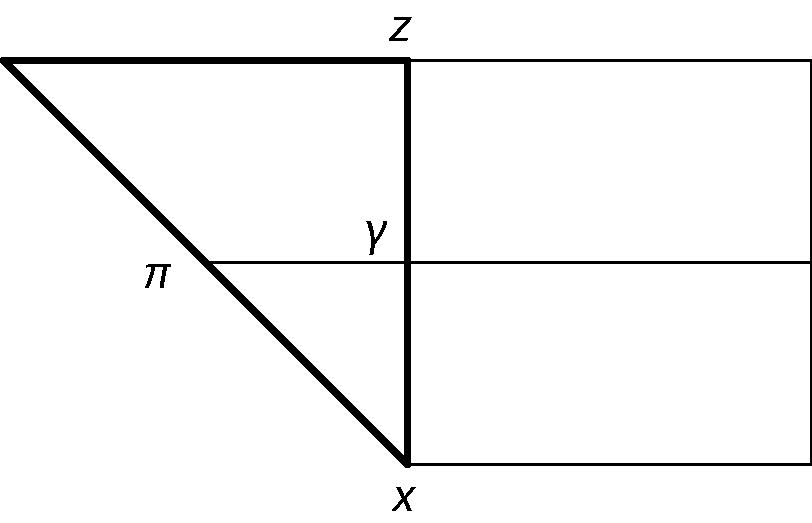
\includegraphics[width=0.28\textwidth]{gesamttex/edit_VIII,3/images/LH_35_09_23_001-002_d3.pdf}} % lh0350923_002r-d4 
\newline%
% \newline%
\centerline{{\normalsize{\lbrack\textit{Fig.~3, gestr.}\rbrack}}}
\newline%
\newline%
% \newline%
{\footnotesize%
\textsuperscript{[a]}~%
\textit{(1)}~\textit{xz} aequ. \textit{a} et
\textit{(a)}~$x\gamma$ aequ.
\textit{(b)}~$\gamma\pi$ aequ. \textit{y}
\textit{(2)}~$z\gamma$%
~\textit{L}
\quad
\textsuperscript{[b]}~differentia
\textit{(1)}~sit \textit{z} aequ.
\textit{(2)}~sit celeritas incursus \textit{e}, erit~%
\textit{L}}%
}}}
\pend%
% \newpage%
%
\pstart%
Linea%
\edlabel{LH_35_09_23_002r_probaturrecta_mxyz-1}
$\beta\delta x$ est recta
seu celeritas%
\protect\index{Sachverzeichnis}{celeritas corporis incurrentis}
%
\edtext{incurrentis}{%
\lemma{incurrentis}\Bfootnote{%
\textit{erg.~L}}}
%
residua uniformiter
%
\edtext{minuitur pro magnitudine%
\protect\index{Sachverzeichnis}{magnitudo corporis}
corporis excipientis aucta,%
\protect\index{Sachverzeichnis}{corpus excipiens}
sive celeritates residuae%
\protect\index{Sachverzeichnis}{celeritas residua}
$\gamma\delta$, $\textit{(}\gamma\textit{)(}\delta\textit{)}$%
}{%
\lemma{minuitur}\Bfootnote{%
\textit{(1)}~resistentia
\textit{(2)}~res
\textit{(3)}~pro magnitudine corporis \textbar\ excipientis \textit{erg.} \textbar\ aucta, sive
\textit{(a)}~ea est
\textit{(b)}~pro au
\textit{(c)}~celeritates residuae
\textit{(aa)}~ejusdem corporis incurrentis sunt
\textit{(bb)}~ut differ
\textit{(cc)}~ad
\textit{(dd)}~inter se
\textit{(ee)}~$\gamma\delta$, $\textit{(}\gamma\textit{)(}\delta\textit{)}$%
~\textit{L}}}
%
ejusdem corporis incurrentis%
\protect\index{Sachverzeichnis}{corpus incurrens}
ut \textit{xz}
in diversa excipientia
ut $z\gamma, z\textit{(}\gamma\textit{)}$
erunt inter se
ut ipsae $x\gamma, x\textit{(}\gamma\textit{)}$
excessus corporis incurrentis
super excipientia.%
\pend%
%
\pstart%
\edtext{%
Haec propositio%
\protect\index{Sachverzeichnis}{propositio}
patet ex ipsa
%
\edtext{progressionis%
\protect\index{Sachverzeichnis}{progressio simplex}
simplicitate,%
\protect\index{Sachverzeichnis}{simplicitas progressionis}%
}{%
\lemma{\textit{Über} progressionis simplicitate \textit{zwischenzeilig:}}\Afootnote{%
Imo non est simplex
sed plura consideranda.%
\newline}}
%
ubi non potest locum habere
nisi vel hyperbola%
\protect\index{Sachverzeichnis}{hyperbola}
vel recta.%
\protect\index{Sachverzeichnis}{linea recta}
%
\edtext{%
Hyperbola%
\edtext{ autem non potest,
ut tentanti patebit,}{%
\lemma{\textit{Über} Hyperbola \lbrack...\rbrack\ patebit \textit{zwischenzeilig}:}\Afootnote{%
Imo est hyperbola%
\protect\index{Sachverzeichnis}{hyperbola}
sed componuntur duarum hyperbolarum ordinatae.%
}}
%
deberet enim in ea $z\beta$ fieri infinita
seu asymptotos.\protect\index{Sachverzeichnis}{asymptotos}%
}{%
\lemma{Hyperbola \lbrack...\rbrack\ asymptotos}\Cfootnote{%
Siehe über dieses Missverständnis \textsc{Fichant} 1994, S.~198.\cite{01056}}}
%
Non itaque dici potest celeritates%
\protect\index{Sachverzeichnis}{celeritas corporis incurrentis}
%
\edtext{incurrentis}{%
\lemma{incurrentis}\Bfootnote{%
\textit{erg.~L}}}
%
residuas esse in reciproca corporum%
\protect\index{Sachverzeichnis}{corpus excipiens}
%
\edtext{excipientium}{%
\lemma{excipientium}\Bfootnote{%
\textit{erg.~L}}}
%
magnitudine,\protect\index{Sachverzeichnis}{magnitudo corporis}
nam
%
\edtext{ita corpore excipiente existente}{%
\lemma{ita}\Bfootnote{%
\textit{(1)}~celeritate
\textit{(2)}~corpore
\textit{(a)}~existente
\textit{(b)}~excipiente existente%
~\textit{L}}}
%
minimo fieret
%
\edtext{celeritas incurrentis%
\protect\index{Sachverzeichnis}{celeritas corporis incurrentis}
infinita,}{%
\lemma{celeritas}\Bfootnote{%
\textit{(1)}~excipientis infi
\textit{(2)}~incurrentis infinita,~%
\textit{L}}}
%
quae tamen finita est,
manet scilicet qualis
% \edlabel{LH_35_09_23_001-002_concursu5}% % ex-label: concusrsus5
erat.%
\edlabel{LH_35_09_23_002r_probaturrecta_mxyz-2}%
}{%
\lemma{\textit{Am Rand:}}\Afootnote{%
Videamus quae fiat linea,
si residuum in incurrente\protect\index{Sachverzeichnis}{corpus incurrens}
sit ad incursum,
ut corporum differentia ad summam.%
\protect\index{Sachverzeichnis}{summa corporum}%
\protect\index{Sachverzeichnis}{differentia corporum}
Sit corpus majus constans \textit{m},
corpus minus sit $\mu,$
quod variare ponatur,
incursus\protect\index{Sachverzeichnis}{incursus}
sit autem certus
et idem \textit{e},\textsuperscript{[a]}
et residua incurrentis celeritas quaeritur $\epsilon,$
fiet:
$\displaystyle\frac{\epsilon}{e}$ aequ.
$\displaystyle\frac{m-\mu}{m+\mu}$
seu $\epsilon$ aequ. $\displaystyle\frac{m-\mu}{m+\mu}e,$
quae aequatio,%
\protect\index{Sachverzeichnis}{aequatio}
positis \textit{m,} \textit{e} constantibus
et $\mu,$ $\epsilon$ variatis,
est ad hyperbolam.\protect\index{Sachverzeichnis}{hyperbola}
Ponatur $m - \mu$ aequ. \textit{d},
fiet $\mu$ aequ. $m - d$
adeoque fiet $\epsilon$ aequ. $\displaystyle\frac{d}{2m-d}e$
quam ad hyperbolam%
\protect\index{Sachverzeichnis}{hyperbola}
esse patet.
Hanc autem veram esse lineam suo loco\textsuperscript{[b]} demonstrabitur,
non rectam.%
\protect\index{Sachverzeichnis}{linea recta}%
\newline%
\newline%
{\footnotesize%
\textsuperscript{[a]}~idem \textit{e},
\textit{(1)}~ponatur
\textit{(2)}~et residua \lbrack...\rbrack\ quaeritur $\epsilon$~% incurrentis celeritas
\textit{L}
\quad
\textsuperscript{[b]}~suo loco\,: Nicht ermittelt.
In N.~\ref{dcc_05}, %??S01\textsubscript{6}, 
Randbemerkung zu S.~\refpassage{LH_35_09_23_012v_sbchj-1}{LH_35_09_23_012v_sbchj-2}
hält Leibniz erstmals fest,
dass die Linie $\displaystyle\beta\delta\textit{(}\delta\textit{)}x$ keine Gerade sein kann.%
}%
\newline}}
% \edtext{}{{\xxref{LH_35_09_23_001-002_concursu5}{{LH_35_09_23_001-002_concursu6}}\lemma{erat.}\Bfootnote{%
% \textit{(1)}~Pro
% \textit{(2)}~Celeritas%
% ~\textit{L}}}}%
\pend%
\newpage%
%
\pstart%
\edtext{Celeritas%
\edlabel{LH_35_09_23_002r_majausinminus_bfnd-1}
% \edlabel{LH_35_09_23_001-002_concursu6} % % ex-label: concursus6
%
residua%
\protect\index{Sachverzeichnis}{celeritas residua}%
\protect\index{Sachverzeichnis}{celeritas corporis incurrentis}
%
\edtext{$\gamma\delta$}{%
\lemma{$\gamma\delta$}\Bfootnote{%
\textit{erg.~L}}}
%
corporis \textit{zx} incurrentis%
\protect\index{Sachverzeichnis}{corpus incurrens}
in aliud minus
%
\edtext{$z\gamma,$}{%
\lemma{$z\gamma$}\Bfootnote{%
\textit{erg.~L}}}
%
est ad celeritatem incursus $z\beta$,%
\protect\index{Sachverzeichnis}{celeritas incursus}
ut differentia corporum $x\gamma$
est ad corpus majus
sive incurrens \textit{xz}.
Patet ex praecedenti.%
\edlabel{LH_35_09_23_002r_majausinminus_bfnd-2}%
}{%
\lemma{\textit{Am Rand:}}\Afootnote{%
Vis progressus\protect\index{Sachverzeichnis}{vis progressus}
incurrentis\textsuperscript{[a]}
crescit pro incremento ejus supra aequalitatem.
Vis impulsus\protect\index{Sachverzeichnis}{vis impulsus}
recepti ab excipiente%
\protect\index{Sachverzeichnis}{corpus excipiens}
crescit\textsuperscript{[b]}
pro incremento ejus versus aequalitatem.%
\newline%
\newline%
{\footnotesize%
\textsuperscript{[a]}~incurrentis
\textit{erg.~L}
\quad
\textsuperscript{[b]}~crescit
\textit{(1)}~cum ejus magnitudine
\textit{(2)}~pro incremento ejus%
~\textit{L}}%
\newline}}%
%
\edtext{}{%
\lemma{\textit{Am Ende des Absatzes, zwischenzeilig:}}\Afootnote{%
Error: non est linea recta.%
\protect\index{Sachverzeichnis}{linea recta}}}%
%
\pend%
%
\pstart%
Corpus excipiens%
\protect\index{Sachverzeichnis}{corpus excipiens}
%
\edtext{minus accipit}{%
\lemma{minus}\Bfootnote{%
\textit{(1)}~residuam
\textit{(2)}~accipit%
~\textit{L}}}
%
vim%
\protect\index{Sachverzeichnis}{vis perdita}
%
\edtext{ab incurrente%
\protect\index{Sachverzeichnis}{corpus incurrens}
perditam}{%
\lemma{ab}\Bfootnote{%
\hspace{-0,5mm}incurrente perditam
\textit{erg.~L}}}
%
sed celeritate%
\protect\index{Sachverzeichnis}{celeritas corporis excipientis}
fertur tanto majore,
quanto ipsum incurrente minus est.
Patet:
alioqui non servaretur vis eadem in summa%
\protect\index{Sachverzeichnis}{summa virium}.
%
\lbrack2~v\textsuperscript{o}\rbrack\
%
\pend%
\pstart%
\noindent%
\hspace{-3,0mm}
$\begin{array}[t]{ccccc}
A\textit{(A)}\ 6 & AC\ 2 & C\textit{(C)}\ 4 & \textit{(A)}\textit{((A))}\ 3 & \textit{(B)}\textit{((B))}\ 6 \\
\textit{(B)} & & \textit{(A)} & & \\
\textit{(C)} & & B & & \\
B & & \textit{(B)} & & \\
\end{array}$
% \edtext{}{%
% \lemma{}\Bfootnote{%
% \textit{(1)}~Si
% \textit{(2)}~$A (A) 6$%
% ~\textit{L}}}%
\pend%
%
\pstart%
\noindent%
Ergo \textit{((A))((B))} 3. \textit{((A))((C))} 1. \textit{(C)((A))} aequ. \textit{(A)((A))}
%
\edtext{aequ. 3. et \textit{(C)((C))}}{%
\lemma{aequ.}\Bfootnote{%
\hspace{-0,5mm}3.
\textbar~et \textit{gestr.}~%
\textbar\ et \textit{(C)((C))}%
~\textit{L}}}
%
\mbox{aequ.}
\raisebox{-2,22mm}{$\displaystyle\efrac{\textit{(C)((A))}}{3} +\displaystyle\efrac{\textit{((A))((C))}}{1}$}.
Ergo \textit{(C)((C))} aequ. 4 aequ. \textit{C(C)}.
% \pend%
%
% \pstart%
Hinc patet
viam centri gravitatis%
\protect\index{Sachverzeichnis}{centrum gravitatis}%
\protect\index{Sachverzeichnis}{via centri gravitatis}
hoc modo manere eandem.%
\rule[-0mm]{0mm}{4mm}
\pend%
%%
%  \newpage% 
 \vspace{4.5em}%	% Diagramm 4
  \centerline{\includegraphics[width=0.93\textwidth]{gesamttex/edit_VIII,3/images/LH_35_09_23_001-002_d4.pdf}}%
  \vspace*{0.5em}
  \centerline{\lbrack\textit{Fig.~4}\rbrack}%
  \label{LH_35_09_23_001-002_Fig.4}%
  %\vspace{1.5em}%
 \newpage%
%
\pstart%
\edtext{Calculo generaliore,%
\protect\index{Sachverzeichnis}{calculus generalior}%
}{%
\lemma{\textit{Am Rand:}}\Afootnote{errores%
\protect\index{Sachverzeichnis}{error}
\newline}}
%
\rule[-2mm]{0mm}{8mm}%
%
% \quad%
\textit{A(A)} aequ. \textit{A(C)} aequ. \textit{AB} aequ. \textit{A(B)}
%
\edtext{sit}{%
\lemma{sit}\Bfootnote{\hspace{-0,5mm}%
\textit{erg.~L}}}
%
aequ.
%
\edtext{\textit{e}.}{%
\lemma{\textit{Am Rand, auf die Größe e bezogen:}}\Afootnote{$e + \phantom{e}$}}
%
\quad%
\textit{AC} sit ad \textit{CB},
ut \textit{b} ad \textit{a}.
$\displaystyle\frac{AC}{CB} \sqcap \displaystyle\frac{b}{a}.$
\rule[-4mm]{0mm}{10mm}%
% \quad%
Ergo \textit{AC} aequ. $\displaystyle\frac{b}{a+b}e$
et \textit{BC} aequ. $\displaystyle\frac{a}{a+b}e.$
\edlabel{LH_35_09_23_002v_C(C)Wert_asfd-1}%
\textit{C(C)} aequ. $e-\displaystyle\frac{b}{a+b}e,$
aequ. $\displaystyle\frac{ae+be-be}{a+b}$
aequ. $\displaystyle\frac{ae}{a+b}$.%
\edlabel{LH_35_09_23_002v_C(C)Wert_asfd-2}
\quad%
% \rule[-4mm]{0mm}{10mm}%
% \raisebox{-2,22mm}{
$\underset{\displaystyle\epsilon\phantom{ll}}{\displaystyle\textit{(A)((A))}}$
% }
ad 
% \raisebox{-2,22mm}{
$\underset{\displaystyle e\phantom{l}}{\displaystyle\textit{A(A)}}$
% }
ut $a - b$ ad \textit{a}.
\rule[-4mm]{0mm}{10mm}%
% \quad%
Ergo $\epsilon$ aequ. $\displaystyle\frac{a-b}{a}e,$
seu $e-\displaystyle\frac{b}{a}e$ aequ. $\textit{(A)((A))}.$
\rule[-5mm]{0mm}{3mm}%
\quad%
\edlabel{LH_35_09_23_002v_(B)((B))-Wert_jhsb-1}%
Sed \textit{(B)((B))} celeritas ipsius \textit{b}%
\protect\index{Sachverzeichnis}{celeritas corporis excipientis}
quam vocabimus \textit{y},
ducta in \textit{b}
facit \textit{yb} vim ipsi \textit{B} communicatam,%
\protect\index{Sachverzeichnis}{vis communicata}
quae aequatur ipsi \textit{ae}
seu vi priori ipsius \textit{A},
substracta vi residua,\protect\index{Sachverzeichnis}{vis residua}
nempe $ae - be,$
est ergo illa vis $ae, -\, ae + be$
seu est \textit{be},
ergo \textit{be} aequ. \textit{yb}
seu \textit{y} aequ. \textit{e}
%
\edtext{aequ. \textit{(B)((B))}.}{%
\lemma{aequ.}\Bfootnote{\hspace{-0,5mm}%
\textit{(B)((B))}
\textit{erg.~L}}}%
\edlabel{LH_35_09_23_002v_(B)((B))-Wert_jhsb-2}
%
\pend%
%
\pstart%
Hinc
%
\edtext{corpus majus incurrens%
\protect\index{Sachverzeichnis}{corpus incurrens}}{%
\lemma{corpus}\Bfootnote{%
\textit{(1)}~incurrens
\textit{(2)}~majus incurrens%
~\textit{L}}}
%
minori quiescenti%
\protect\index{Sachverzeichnis}{corpus quiescens}
eam quam habebat ipsi tribuit cele\-ri\-ta\-tem%
\protect\index{Sachverzeichnis}{celeritas corporis incurrentis}
(\protect\vphantom)%
quamvis non eam quam habebat ipsi tribuat vim.%
\protect\index{Sachverzeichnis}{vis corporis incurrentis}%
\protect\vphantom()
\pend%
  \vspace{4.0em}%	% Diagramm 5
  \centerline{\includegraphics[width=0.88\textwidth]{gesamttex/edit_VIII,3/images/LH_35_09_23_001-002_d5.pdf}}%
  \vspace*{0.5em}
  \centerline{\lbrack\textit{Fig.~5}\rbrack}%
  \label{LH_35_09_23_001-002_Fig.5}%
 \newpage
%
\pstart%
\edtext{Porro}{%
\lemma{\textit{Am Rand:}}\Afootnote{%
\lbrack\textsuperscript{[a]}%
Nota quantum intersit inter transpositionem%
\protect\index{Sachverzeichnis}{transpositio}
ut substractio\protect\index{Sachverzeichnis}{subtractio}
appareat,
nam \textit{((A))((B))} aequ. $\textit{(A)((B))} - \textit{(A)((A))}.$
non aeque apparet ex literis at \textit{((A))((B))} aequ. $\textit{((B))(A)} - \textit{(A)((A))}.$%
\rbrack\textsuperscript{[b]}%
\protect\index{Sachverzeichnis}{litera}%
\newline\vspace{-0.5em}%
\newline%
{\footnotesize%
\textsuperscript{[a]}~Eckige Klammer von Leibniz.
\quad
\textsuperscript{[b]}~Eckige Klammer vom Hrsg.}%
\newline}}
%
\textit{((A))((B))} % \! 
aequ. % \!\! %%%%%
%\raisebox{-4,20mm}{$\displaystyle\efrac{\textit{((B))(A)}-\textit{(A)((A))}}{\displaystyle\efrac{\textit{(B)}\hspace{9mm}}{\hspace{7,0mm}e\hspace{7mm}\overline{1-\displaystyle\frac{b}{a}e}}}$}.
$\underset{%
\underset{\displaystyle\phantom{\textit{((B))}}e\vphantom{\displaystyle\frac{a}{b}}}%
{\displaystyle\textit{\phantom{((B))}(B)}}}%
{\displaystyle\textit{((B))(A)}}
-
\underset{%
\underset{\displaystyle\overline{1-\displaystyle\frac{b}{a}}\:e}%
{\displaystyle\phantom{\textit{aaaa}}}}
{\displaystyle\textit{(A)((A))}}.$
% \pend%
% \pstart%
% \quad
Ergo \textit{((A))((B))} aequ. $\displaystyle\frac{b}{a}e,$
%\rule[-5mm]{0mm}{4mm}%
et \textit{((B))((C))}\, aequ. $\displaystyle\frac{a}{a+b}\smallfrown\displaystyle\frac{b}{a}e.$
% \pend%
% \pstart%
% \quad
Ergo fiet \textit{((B))((C))} aequ. $\displaystyle\frac{b}{a+b}e$
%
\edtext{aequ. \textit{AC}}{%
\lemma{\textit{Unter} aequ. \textit{AC:}}\Afootnote{(mirum)
\newline}}
%
et \textit{(C)((C))} aequ. $\textit{(B)((B))} - \textit{((B))((C))}$
aequ. $e-\displaystyle\frac{b}{a+b}e$
aequ. $\displaystyle\frac{ae}{a+b}$%
\rule[-5mm]{0mm}{4mm}
\edtext{ut ante.}{%
\lemma{ut ante}\Cfootnote{%
Vgl. S.~\refpassage{LH_35_09_23_002v_C(C)Wert_asfd-1}{LH_35_09_23_002v_C(C)Wert_asfd-2}.}}
%
\edtext{}{%
\lemma{\textit{Am Rand:}}\Afootnote{%
Corpora sumsi ut in puncto consistentia,
ut \textit{(A), (B), (C)} coincidant;
quia alias\textsuperscript{[a]}
calculando comperi\textsuperscript{[b]}
dimensionis ipsorum sive extensionis expressiones
inter calculandum evanescere,
et semper prodire idem;
itaque compendio uti volui.
\newline\vspace{-0.5em}%
\newline%
{\footnotesize%
\textsuperscript{[a]}~alias:
Vgl. etwa N.~\ref{RK57276}, %??M10 = Centrum gravitatis semper sequitur
\refpassage{LH_37_05_149r_pnctmtrl-1}{LH_37_05_149r_pnctmtrl-2}.
\quad
\textsuperscript{[b]}~comperi
\textit{(1)}~\textlangle\textendash\textrangle\
\textit{(2)}~etiamsi magnitudinis ipsorum consideratio
\textit{(3)}~dimensionis ipsorum%
~\textit{L}%
\newline}}}%
\label{LH_35_09_23_002v_MargCoincidunt}
%
\pend%
%
\pstart%
Hinc ergo praeclara ducimus
\label{LH_35_09_23_001-002_theoremata}% % ex-label: theoremata
%
\edtext{theoremata,%
\protect\index{Sachverzeichnis}{theorema praeclarum}
\edlabel{LH_35_09_23_002v_majusinminquiesc_jksr-1}%
in hoc casu corporis majoris
in minus quiescens%
\protect\index{Sachverzeichnis}{corpus quiescens}
incurrentis,%
\protect\index{Sachverzeichnis}{corpus incurrens}
centrum gravitatis%
\protect\index{Sachverzeichnis}{centrum gravitatis}}{%
\lemma{theoremata,}\Bfootnote{%
\textit{(1)}~centrum grav
\textit{(2)}~in hoc \lbrack...\rbrack\ centrum gravitatis%
~\textit{L}}}
%
eadem progredi celeritate%
\protect\index{Sachverzeichnis}{celeritas centri gravitatis}
%
\edtext{\lbrack et\rbrack}{%
\lemma{et}\Bfootnote{%
\textit{erg.~Hrsg.}}}
%
\edlabel{LH_35_09_23_002v_majusinminquiesc_jksr-3}%
distantiam%
\protect\index{Sachverzeichnis}{distantia ante concursum}
%
\edtext{corporum ante concursum esse ad distantiam eodem tempore
(\protect\vphantom)%
quantum concursui insumtum erat%
\protect\vphantom()
post}{%
\lemma{corporum}\Bfootnote{%
\textit{(1)}~aequali tempore post
\textit{(2)}~ante concursum \lbrack...\rbrack\ erat%
\protect\vphantom() post%
~\textit{L}}}
%
\protect\index{Sachverzeichnis}{distantia post concursum}
concursum acquisitam
ut corpus incurrens%
\protect\index{Sachverzeichnis}{corpus incurrens}
ad excipiens%
\protect\index{Sachverzeichnis}{corpus excipiens}.%
\edlabel{LH_35_09_23_002v_majusinminquiesc_jksr-2}
(\protect\vphantom)%
Hinc cum aequalia sunt%
\protect\index{Sachverzeichnis}{corpora aequalia}
fit eadem%
\protect\vphantom().
Denique corporis excipientis distantia a centro gravitatis%
\protect\index{Sachverzeichnis}{centrum gravitatis}%
\protect\index{Sachverzeichnis}{distantia a centro gravitatis}
post concursum aequatur distantiae corporis
%
\edtext{incurrentis a centro gravitatis ante concursum.}{%
\lemma{incurrentis}\Bfootnote{%
\textit{(1)}~ab eadem
\textit{(2)}~ante concursum
\textit{(3)}~a centro gravitatis ante concursum.%
~\textit{L}}}%
%
\edtext{}{%
\lemma{\textit{Am Ende des Absatzes, zwischenzeilig:}}\Afootnote{errores%
\protect\index{Sachverzeichnis}{error}\vspace{-3mm}%
}}%
%
\pend%
\newpage
%
\pstart%
\edtext{Si%
\edlabel{LH_35_09_23_002v_fkdk-1} corpus incurrat%
\protect\index{Sachverzeichnis}{corpus incurrens}
in minus antecedens%
\protect\index{Sachverzeichnis}{corpus antecedens}
dabit illi suam
%
\edtext{celeritatem.%
\protect\index{Sachverzeichnis}{celeritas corporis incurrentis}
Nam}{%
\lemma{\textit{Über} celeritatem. Nam \textit{zwischenzeilig}:}\Afootnote{error%
\protect\index{Sachverzeichnis}{error}%
\newline}}
%
quatenus communi feruntur celeritate,%
\protect\index{Sachverzeichnis}{celeritas communis}
eam retinent ambo,
velut si in navi\protect\index{Sachverzeichnis}{navis}
%
\edtext{ferrentur;
at celerius sive insequens%
\protect\index{Sachverzeichnis}{corpus insequens}
intelligi potest
in illa navi
ferri differentia celeritatum,%
\protect\index{Sachverzeichnis}{differentia celeritatum}}{%
\lemma{ferrentur;}\Bfootnote{%
\textit{(1)}~quatenus vero in celeriore sive insequente fertur differentia celeritatum exc
\textit{(2)}~at celerius \lbrack...\rbrack\ differentia celeritatum,%
~\textit{L}}}
%
et tardius sive antecedens,%
\protect\index{Sachverzeichnis}{corpus antecedens}
intelligi potest in navi%
\protect\index{Sachverzeichnis}{navis}
quiescere.%
\protect\index{Sachverzeichnis}{corpus quiescens}
Ergo incurrens dabit ipsi suam celeritatem.%
}{%
\lemma{\textit{Am Rand:}}\Afootnote{%
Videndum
an non eodem modo linea recta prodire debeat
quoad motum excipientis.%
\protect\index{Sachverzeichnis}{motus corporis excipientis}
In eo erravimus,
scilicet quod incurrentis quidem\lbrack,\rbrack\
non vero et excipientis\lbrack,\rbrack\
simplicem celeritatis expressionem quaesivimus.
\newline}}
%
Idem vero retinet priorem communem,
cum ergo nunc et sua celeritate priore
et praeterea excessu alterius super suam priorem feratur,
tota celeritate incurrientis feretur.%
\protect\index{Sachverzeichnis}{celeritas corporis incurrentis}%
\edlabel{LH_35_09_23_002v_fkdk-2}
\pend%
%
%
%  \newpage% 
%  \vspace{2.0em}%	% Diagramm 5
%  \centerline{\includegraphics[width=0.86\textwidth]{gesamttex/edit_VIII,3/images/LH_35_09_23_001-002_d5.pdf}}%
%  \vspace*{0.5em}
%  \centerline{\lbrack\textit{Fig.~5}\rbrack}%
%  \label{LH_35_09_23_001-002_Fig.5}%
%  \vspace{1.25em}%
%  \newpage%
%
%
\pstart%
Calculo rem subjici proderit.%
\protect\index{Sachverzeichnis}{calculus}
Corpus \textit{A} aequ. \textit{a},
corpus \textit{B} aequ. \textit{b}.
\textit{A(A)} celeritas
%
\edtext{prior}{%
\lemma{prior}\Bfootnote{\hspace{-0,5mm}%
\textit{erg.~L}}}
%
corporis \textit{a}, sit \textit{e}.
\textit{B(B)} celeritas prior corporis
%
\edtext{\lbrack\textit{b},\rbrack}{%
\lemma{\textit{B}}\Bfootnote{%
\textit{L~ändert Hrsg. nach~E,\cite{01056} S.~78}}}
%
sit \textit{i}.
Erit \textit{AB} distantia corporum%
\protect\index{Sachverzeichnis}{distantia corporum}
aequ. $e - i$
et \textit{AC} aequ. $\displaystyle\frac{b}{a+b}\overline{e-i}$
\rule[-4mm]{0mm}{10mm}%
et \textit{BC} aequ. $\displaystyle\frac{a}{a+b}\overline{e-i}$
\edlabel{LH_35_09_23_002v_utantea_ghfs-1}et $C(C)$ aequ.
%
\edtext{\lbrack$\textit{A(A)} - AC$\rbrack}{%
\lemma{$\textit{A(A)} - \textit{(A)C}$}\Bfootnote{%
\textit{L~ändert Hrsg. nach~E,\cite{01056} S.~78}}}
%
(\protect\vphantom)%
\edlabel{LH_35_09_23_002v_PunctaCoincidunt_wdm-1}%
quia
%
\edtext{ponimus puncta}{%
\lemma{ponimus}\Bfootnote{%
\textit{(1)}~corpora
\textit{(2)}~puncta%
~\textit{L}}}
%
\textit{(A)}, \textit{(B)}, \textit{(C)} coincidere,
seu corpora \textit{A}, \textit{B} in puncto consistere%
\edlabel{LH_35_09_23_002v_PunctaCoincidunt_wdm-2}%
\protect\vphantom()
sive $e-\displaystyle\frac{b}{a+b}\overline{e-i}$%
\rule[-4mm]{0mm}{10mm}
sive $\displaystyle\frac{ae + be-be + bi}{a+b}$ sive $\displaystyle\frac{ae + bi}{a+b}$ aequ. \textit{C(C)}.%
\edlabel{LH_35_09_23_002v_utantea_ghfs-2}%
%
\edtext{}{%
\lemma{\textit{Am Rand:}}\Afootnote{errores}}%
%
\pend%
%
\pstart%
Hinc patet potentiam%
\protect\index{Sachverzeichnis}{potentia corporum concurrentium}
(\protect\vphantom)%
quae est etiam $ae + bi$%
\protect\vphantom()
per summam corporum divisam,%
\protect\index{Sachverzeichnis}{summa corporum}
dare celeritatem centri gravitatis,%
\protect\index{Sachverzeichnis}{celeritas centri gravitatis}
hoc loco.
\edlabel{LH_35_09_23_002v_utostedimus_hik-1}%
Jam \textit{(B)((B))} aequ. \textit{A(A)}
%
\edtext{per hoc loco demonstrata,}{%
\lemma{per \lbrack...\rbrack\ demonstrata}\Cfootnote{%
Siehe S.~\refpassage{LH_35_09_23_002v_(B)((B))-Wert_jhsb-1}{LH_35_09_23_002v_(B)((B))-Wert_jhsb-2}}}
%
ergo \textit{y} aequ. \textit{e}.%
\edlabel{LH_35_09_23_002v_utostedimus_hik-2}
Habetur ergo punctum \textit{((B))},
hinc vero facile invenietur et punctum \textit{((A))}.
Nam quia vis eadem servatur,%
\protect\index{Sachverzeichnis}{vis corporum concurrentium}
ideo ponendo celeritates priores%
\protect\index{Sachverzeichnis}{celeritas ante concursum}
ut dixi \textit{e} et \textit{i},
\makebox[1.0\textwidth][s]{posteriores $\epsilon$ et \textit{y},%
\protect\index{Sachverzeichnis}{celeritas post concursum}
debet esse $ae + bi$ aequ. $a\epsilon + by.$
Id est hoc loco $ae + bi$ aequ. $a\epsilon + be.$}
\pend
\newpage
\pstart
\noindent
Ergo \rule[-4mm]{0mm}{10mm}$\displaystyle\frac{ae + bi-be}{a}$ aequ. $\epsilon$, sive $\epsilon$ aequ.
%
\edtext{$e-\displaystyle\frac{b}{a}\overline{e-i}$ aequ. \textit{(A)((A))},}{%
\lemma{$e-\displaystyle\frac{b}{a}\overline{e-i}$}\Bfootnote{%
\textit{(1)}~. Ergo \textit{((A))((B))}
\textbar~nempe \textit{(B)((B))} $-$ \textit{erg.}~%
\textbar\ erit aequ. $\displaystyle\frac{b}{a}\overline{e-i}$ id est distantia
\textit{(2)}~aequ. \textit{(A)}
\textit{(a)}~\textit{((B))}
\textit{(b)}~\textit{((A))}
\textit{(3)}~aequ. \textit{(A)((A))},%
~\textit{L}}}
%
id est \textit{(A)((A))} aequ. $\textit{(B)((B))} - \displaystyle\frac{b}{a}\overline{e-i},$
% \rule[-4mm]{0mm}{10mm}
at eadem \textit{(A)((A))} aequ. $\textit{(B)((B))} - \textit{((A))((B))}.$
Ergo \textit{((A))((B))} aequ. $\displaystyle\frac{b}{a}\overline{e-i}$%
\rule[-4mm]{0mm}{10mm}
sive distantia corporum post concursum%
\protect\index{Sachverzeichnis}{distantia post concursum}
est ad distantiam corporum ante concursum,%
\protect\index{Sachverzeichnis}{distantia ante concursum}
ut corpus excipiens%
\protect\index{Sachverzeichnis}{corpus excipiens}
ad incurrens,%
\protect\index{Sachverzeichnis}{corpus incurrens}%
\rule[-4mm]{0mm}{8mm}
prorsus quemadmodum
%
\edtext{supra}{\lemma{supra}\Cfootnote{%
S.~\refpassage{LH_35_09_23_002v_majusinminquiesc_jksr-3}{LH_35_09_23_002v_majusinminquiesc_jksr-2}.}}
%
cum excipiens quiescere poneretur.
%
\edtext{Porro \textit{((A))((C))}}{%
\lemma{Porro}\Bfootnote{%
\textit{(1)}~\textit{AC}
\textit{(2)}~\textit{((A))((C))}%
~\textit{L}}}
%
aequ. $\displaystyle\frac{b}{a+b},$ $\overline{\displaystyle\frac{b}{a}\overline{e-i}}$%
\rule[-4mm]{0mm}{10mm}
seu $\displaystyle\frac{b^2}{a^2+ba}\overline{e-i},$
et \textit{((B))((C))} aequ. $\displaystyle\frac{a}{a+b}%
\rule[-4mm]{0mm}{10mm}
\overline{\displaystyle\frac{b}{a}\overline{e-i}}$
aequ. $\displaystyle\frac{b}{a+b}\overline{e-i}$
aequ. \textit{AC}.
Porro \textit{(C)((C))} aequ. $\textit{(B)((B))} - \textit{((B))((C))}$%
\rule[-4mm]{0mm}{10mm}
seu $e-\displaystyle\frac{b}{a+b}\overline{e-i},$
id est \textit{(C)((C))} aequ. $\displaystyle\frac{ae + be-be + bi}{a+b}$,
seu $\displaystyle\frac{ae + bi}{a+b},$%
\rule[-4mm]{0mm}{10mm}
ut
%
\edtext{antea}{\lemma{antea}\Cfootnote{%
S.~\refpassage{LH_35_09_23_002v_utantea_ghfs-1}{LH_35_09_23_002v_utantea_ghfs-2}.}}
%
\textit{C(C)}.
Ergo hic quoque centrum gravitatis\protect\index{Sachverzeichnis}{centrum gravitatis}
eadem qua ante celeritate progreditur.%
\protect\index{Sachverzeichnis}{celeritas centri gravitatis}%
\protect\index{Sachverzeichnis}{progressus centri gravitatis}%
\rule[-4mm]{0mm}{8mm}%
%%%%
    %%%%    ACHTUNG GETRIXT:
\edtext{}{%
\lemma{\hspace{1,6mm}\lbrack\textit{Fig.~6}\rbrack}\killnumber\Cfootnote{%
Das Diagramm ist Gegenstand der \textit{Sche\-da~II};
vgl. N.~\ref{dcc_02-1}, %??S01\textsubscript{2},
S.~\refpassage{LH_35_09_23_003r_BezugFig4_fgkh-1}{LH_35_09_23_003r_BezugFig4_fgkh-2}.
Siehe hierzu \textsc{Fichant} 1994, S.~80.\cite{01056}%
}}
%%%%
\pend%
\count\Bfootins=1200%
\count\Afootins=1200%
\count\Cfootins=1200%
%
%%
%  \newpage% 
  \vspace{2.5em}%	% Diagramm 6
  \centerline{\includegraphics[width=0.87\textwidth]{gesamttex/edit_VIII,3/images/LH_35_09_23_001-002_d6.pdf}}%
  \vspace*{0.5em}
  \centerline{\lbrack\textit{Fig.~6}\rbrack}%
  \label{LH_35_09_23_001-002_Fig.6}%
%  \vspace{1.5em}%
%  \newpage%
%
%
%%%% ENDE des Textes auf Blatt 2v